%% It is just an empty TeX file.
%% Write your code here.
\chapter{Experiment}
\section{Communication Systems}

The goal of the ParSec project is to create a dependable, flexible and secure communication system which meets all industrial automation requirements. It has to work with latencies below 1 ms and with very high noise level, serving many distributed clients at once. Moreover it has to deal with fading effects and potentially many reflections. \autoref{fig:data_path} shows an abstraction of the transmission path, a very common communication model. Although the figure is over 40 years such model is still very up-to-date.
\begin{figure}[H]
\centering
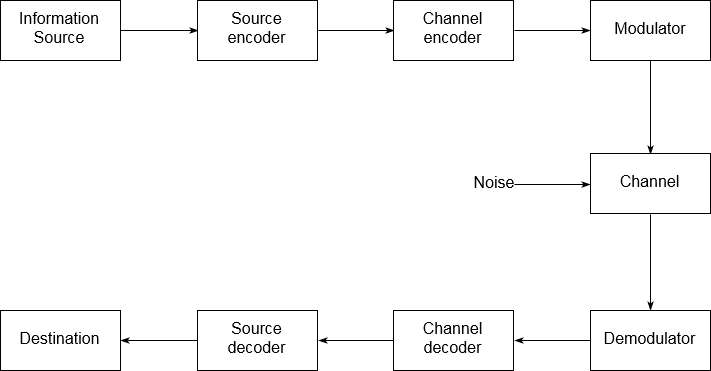
\includegraphics[width=0.65\textwidth]{figures/Data_transmission_path.png}
\caption{Block diagram of a typical data transmission (storage) system~\cite{book:LinCostello}}
\label{fig:data_path}
\end{figure}

The digital source of information can be understood as a MAC layer, followed by:
\begin{itemize}
    \item source encoder - compresses the data by removing useless redundancy, leaving just the information that needs to be transmitted. In other words, a perfectly designed source encoder minimizes the number of bits per unit time needed to represent the source information. Since every bit of compressed information is significant, than decoding a sequence with changed bits would produce catastrophic results.
    \item cryptography encoder - helps to protect the confidentiality and integrity of data being sent, meaning that it cannot be read or altered by unauthorized third parties. It adds useful redundancy to protect the information contained in the message. Cryptography by itself doesn't guarantee any security when not combined with other security means. Without secure key management protocols and thoughtful design the security can be easily compromised. More information can be found in~\cite{Cryptography}. In many cases, one of the encryption stages involves using hash functions which counteracts the manipulation of encrypted bitstream. The hashing algorithm produces a unique output for each individual input, making it impossible to alter the transmitted information without corrupting it. Channing one bit within hashed bitstream leads to decryption of a completely different clear text.
    \item channel encoder - transforms the \textit{information sequence} \textbf{u}, produced by digital source (MAC layer, source encoder or cryptography encoder), into a \textit{code~word} \textbf{v}. It adds useful information redundancy, which despite possible transmission errors, allows the channel decoder to reproduce the information sequence. The simplest example is a parity bit added at the end of a message indicating an odd or even number of ones in the message. More complicated approaches are described in \autoref{sec:coding}.
    \item modulator - since the discrete symbols are not applicable for transmission they need to be translated into the waveform and then sent to the receiver, that's why the channel encoder is followed by the modulator~\cite{book:LinCostello}.
\end{itemize}
All modules come in pairs that are complementary to each other. The demodulators task is to recreate the possible codeword \textbf{v} from the waveform received from the RF module. The channel decoder takes the code word and recreates the information sequence \textbf{u\^}, then the information gets decrypted by cryptography decoder and decoded by source decoder.



%more about baseband processors + graphic
\section{Experiments goal}
Modulators are nowadays parts of the baseband processors, together with frame formatters, DC/AC converters, symbol shaping modules and RF modules~\cite{book:Ismail}. The baseband processors are in fact mixtures of digital and analog components. As mentioned in \autoref{ch:test} the testability of mixed signal components is limited at best. The test has to be conducted outside of such modules.
Hardware faults can happen in the digital logic in the signal path or an error caused by a transient fault in some memory cells storing parity bits. They are all detected and corrected according to the channel coding algorithm. The same applies to permanent faults in hardware, except that they permanently lower the amount of possible transmission errors that can be detected and corrected. The faults also happen in mixed signal modules and analog parts in signal path and they get also corrected 
If there was a possibility to exclude the noisy channel from the communication path, then all detected errors would have to have they origin within the hardware modules, indicating the presence of permanent faults. Such test could happed periodically or during the systems start up.
To implement such solution the transmitter would have to be directly connected with the receiver. Since communication modules are usually designed for both: transmitting and receiving, and all of their components come in complementary pairs, it would be possible to connect the outputs of transmitter modules to corresponding inputs of receivers modules. The idea of such "functional shorts" is shown in \autoref{fig:shorts}.
